\section{Redux} 
\subsection{Overview}
Redux\glosp is a \texttt{npm} module which manage the entire state of the website from client-side. It consists of:
\begin{itemize}
	\item Actions;
	\item Actions Creators;
	\item Reducers;
	\item Store.
\end{itemize}
When the website is built, a default state for the store is set (it is defined into the reducer JavaScript file).
\subsection{Unidirectional pattern} 
Basically some actions are mapped by \texttt{container components} into specific \texttt{presentational components} through them props with \texttt{Connect(arg1, arg2)} method. When a presentational component request a \texttt{dispatch()} of a specific action, a reducer will complete the request by changing the store and returning a new instance of the application state. Each time the store is changed, the \texttt{Render()} method of displayed components is called.
\texttt{Redux} is the name of the pattern implemented by React and Redux, it is an evolution of \texttt{Flux} pattern, the difference is that Flux uses more than one store.\\
\begin{figure}[H]
	\centering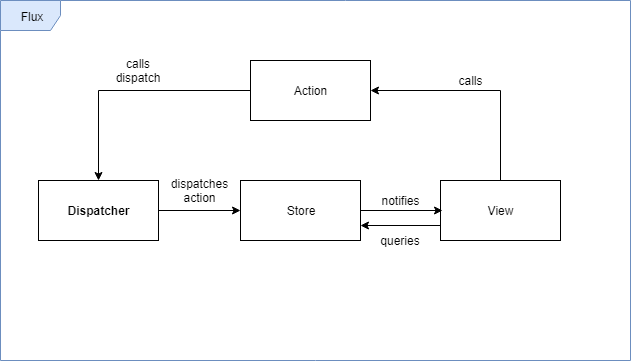
\includegraphics[scale = 0.6]{res/images/Flux.png}
	\caption{Flux pattern}
\end{figure}

\subsection{Actions}
There are seven main categories of actions inside the \texttt{src/actions/} folder. Each action is called by the \texttt{action creator} when a container component request it's dispatch. Here there is the list of actions and what them do when they are invoked.
\begin{itemize}
	\item \textbf{business}: \begin{itemize}
		\item getMyProducts();
		\item getStoreProducts();
		\item setTotalNumberOfProducts();
		\item setTotalNumberOfMyProducts();
		\item passKeyProd();
		\item setInvoices();
		\item setPeriods();
		\item selectedPeriod();
		\item resetInvoices().
	\end{itemize}
	\item \textbf{cart}:
	\begin{itemize}
		\item addToCart();
		\item removeFromCart();
		\item increaseQuantity();
		\item decreaseQuantity();
		\item cartToOrders();
		\item resetCart().
	\end{itemize}
	\item \textbf{government}:
	\begin{itemize}
		\item getCitizenList();
		\item getBusinessList();
		\item getGovernmentBalanceAndTotalAmount();
		\item setVATrefund();
		\item setStatus();
		\item resetPeriod();
		\item setPeriod();
		\item resetVATPeriods();
		\item setVATPeriod();
		\item resetVAT().
	\end{itemize}
	\item \textbf{login}:
	\begin{itemize}
		\item logIn();
		\item logOut();
		\item beginLoading();
		\item endLoading().
	\end{itemize}
	\item \textbf{searchaction}:
	\begin{itemize}
		\item searchaction();
	\end{itemize}
	\item \textbf{store}:
	\begin{itemize}
		\item increaseIndex();
		\item decreaseIndex();
		\item resetIndex().
	\end{itemize}
	\item \textbf{user}:
	\begin{itemize}
		\item getMyProducts();
		\item setLoadingMessage().
	\end{itemize}
\end{itemize}

\subsection{Actions Creators}
There are three different type of Actions Creator. Each of them interacts with Facade (cf. §9) and returns to the related contanier a specific action otherwise rejects an error.
\begin{itemize}
	\item \textbf{Business actions creator} that contains the following functions: 
	\begin{itemize}
		\item getStoreProducts(): returns an action that generates a list of products on sale and returns it as param by returning a redux action;
		\item getMyProducts():
		returns an action that generates a list of products on sale that were added to sell by current logged business and returns it as param by returning a redux action;
		\item addProduct():
		returns an action that adds a product to the store;
		\item modifyProduct():
		returns an action that modifies a product to the store;
		\item deleteProduct():
		returns an action that removes a product from the store;
		\item getTotalStoreProduct():
		returns an action that gets the number of total products into the store;
		\item getTotalMyProduct():
		returns an action that gets the number of total products into the store that were added to sell by current logged business;
		\item getInvoices(): returns an action that gets all the invoices in a quarter;
		\item getBusinessPeriod():
		returns an action that gets all the invoices in a quarter related to the current logged business;
		\item payVATPeriod():
		returns an action that executes the instant payment for a quarter to the government;
		\item putOnHoldVATPeriod(): returns an action that defers the debt of a quarter to the next quarter.
	\end{itemize}
	\item \textbf{User actions creator} that contains the following functions:
	\begin{itemize}
		\item getOrdersList(): returns an action that sets into the redux store all the orders.
	\end{itemize}
	\item \textbf{Government actions creator} that contains the following functions:
	\begin{itemize}
		\item getUserList(): returns an action that sets into the redux store the list of all registered users;
		\item setVATrefund(): returns an action that sets into the redux store an array of the business with the VAT quarter info;
		\item getVATPeriods(): returns an action that gets the list of all quarters;
		\item getBalanceAndTotalAmount(): returns an action that gets the government current balance in Cubit\glosp and the total amount;
		\item mint(): returns an action that mints an amount of Cubit\glo;
		\item distribute(): returns an action that distributes an amount of Cubit\glosp to a specific address;
		\item changeUserState(): returns an action that enables or disables a user;
		\item refund(): returns an action that refunds a business period;
		\item resetPeriods(): returns an action that resets the list of periods into the redux store;
		\item resetVAT(): returns an action that resets the invoices list into the redux store;
		\item resetSearch(): returns an action that resets the searched string into the redux store;
		\item resetPeriod(): returns an action that resets the selected period into the redux store;
		\item setStatus(): returns an action that sets a specific status into the redux store, for optimizing the search of the VAT list.
	\end{itemize}
\end{itemize}
\subsection{Reducers}
\begin{itemize}
	\item \textbf{ReducerAuth}: it makes the dispatch of the actions inside \texttt{actions/login.js};
	\item \textbf{ReducerSearch}: it makes the dispatch of the actions inside \texttt{actions/searchaction.js};
	\item \textbf{ReducerCart}: it makes the dispatch of the actions inside \texttt{actions/cart.js};
	\item \textbf{ReducerGovernment}: it makes the dispatch of the actions inside \texttt{actions/government.js};
	\item \textbf{ReducerBusiness}: it makes the dispatch of the actions inside \texttt{actions/business.js};
	\item \textbf{ReducerStore}: it makes the dispatch of the actions inside \texttt{actions/store.js};
	\item \textbf{ReducerUser}: it makes the dispatch of the actions inside \texttt{actions/user.js}.
\end{itemize}
\subsection{Store}
It's configuration resides into root reducer file, the initial configuration is:
\begin{itemize}
	\item logged: false;
	
	\item user: null;
	
	\item searchProduct: "";
	
	\item cart: [];
	
	\item pending: [];
	
	\item ordersList: [];
	
	\item loading: false;
	
	\item userList: [];
	
	\item myProductsArray: [];
	
	\item index: defaultIndex;
	
	\item totalStoreProduct: 0;
	
	\item totalMyProduct: 0;
	
	\item editProd: null;
	
	\item periods: [];
	
	\item invoices: [];
	
	\item selectedPeriod: {id: "Select a quarter"; amount: null; payable: false};
	
	\item VATRefundList: [];
	
	\item selectedStatus: "";
	
	\item VATPeriods: [];
	
	\item loadingMessage: "".
\end{itemize}
Each time the page is reloaded, the initial configuration of the store is set.

\subsection{Redux-Persist}
It is a \texttt{npm} module used for maintaining the current store even if the user leaves the website. It is browser-locally saved, so if a user will enter into the website from another device or from another browser, the store will be set with default values. It has a blacklist for bypassing some values, in this way reloading the website, these values will not be saved (the blacklist is defined into reducer JavaScript file).

\subsection{How to extend with new Redux features}
To implement a new feature with redux store you have to:
\begin{itemize}
	\item insert a new field inside the initial state of the application, you have to set it into the \texttt{reducers/index.js};
	\item create a new action type inside \texttt{constants/actionTypes.js};
	\item create a new action into a specific file that you can find inside \texttt{action/};
	\item create a new function into the appropriate actions creator that returns the action that was created before. If actions creator doesn't exist, create also a new actions creator (\texttt{actionsCreator/});
	\item insert a new reducer into \texttt{reducers/index.js}, it fetches the action and changes the field created before;
	\item map the actions creator with \texttt{mapDispatchToProps()} to the props of the component and also map the field of the state with \texttt{mapStateToProps()}, then connect them to a react component through \texttt{connect(mapStateToProps, mapDispatchToProps)(component)};
	\item call the actions creator inside the \texttt{mapDispatchToProps()} and with returned action, dispatch it for changing the state of the application, you can check the changed field by accessing it from the component with \texttt{this.props.fieldname}. 
\end{itemize}

\begin{landscape}
	\subsection{UML} 
	
	\begin{figure}[H]
		\centering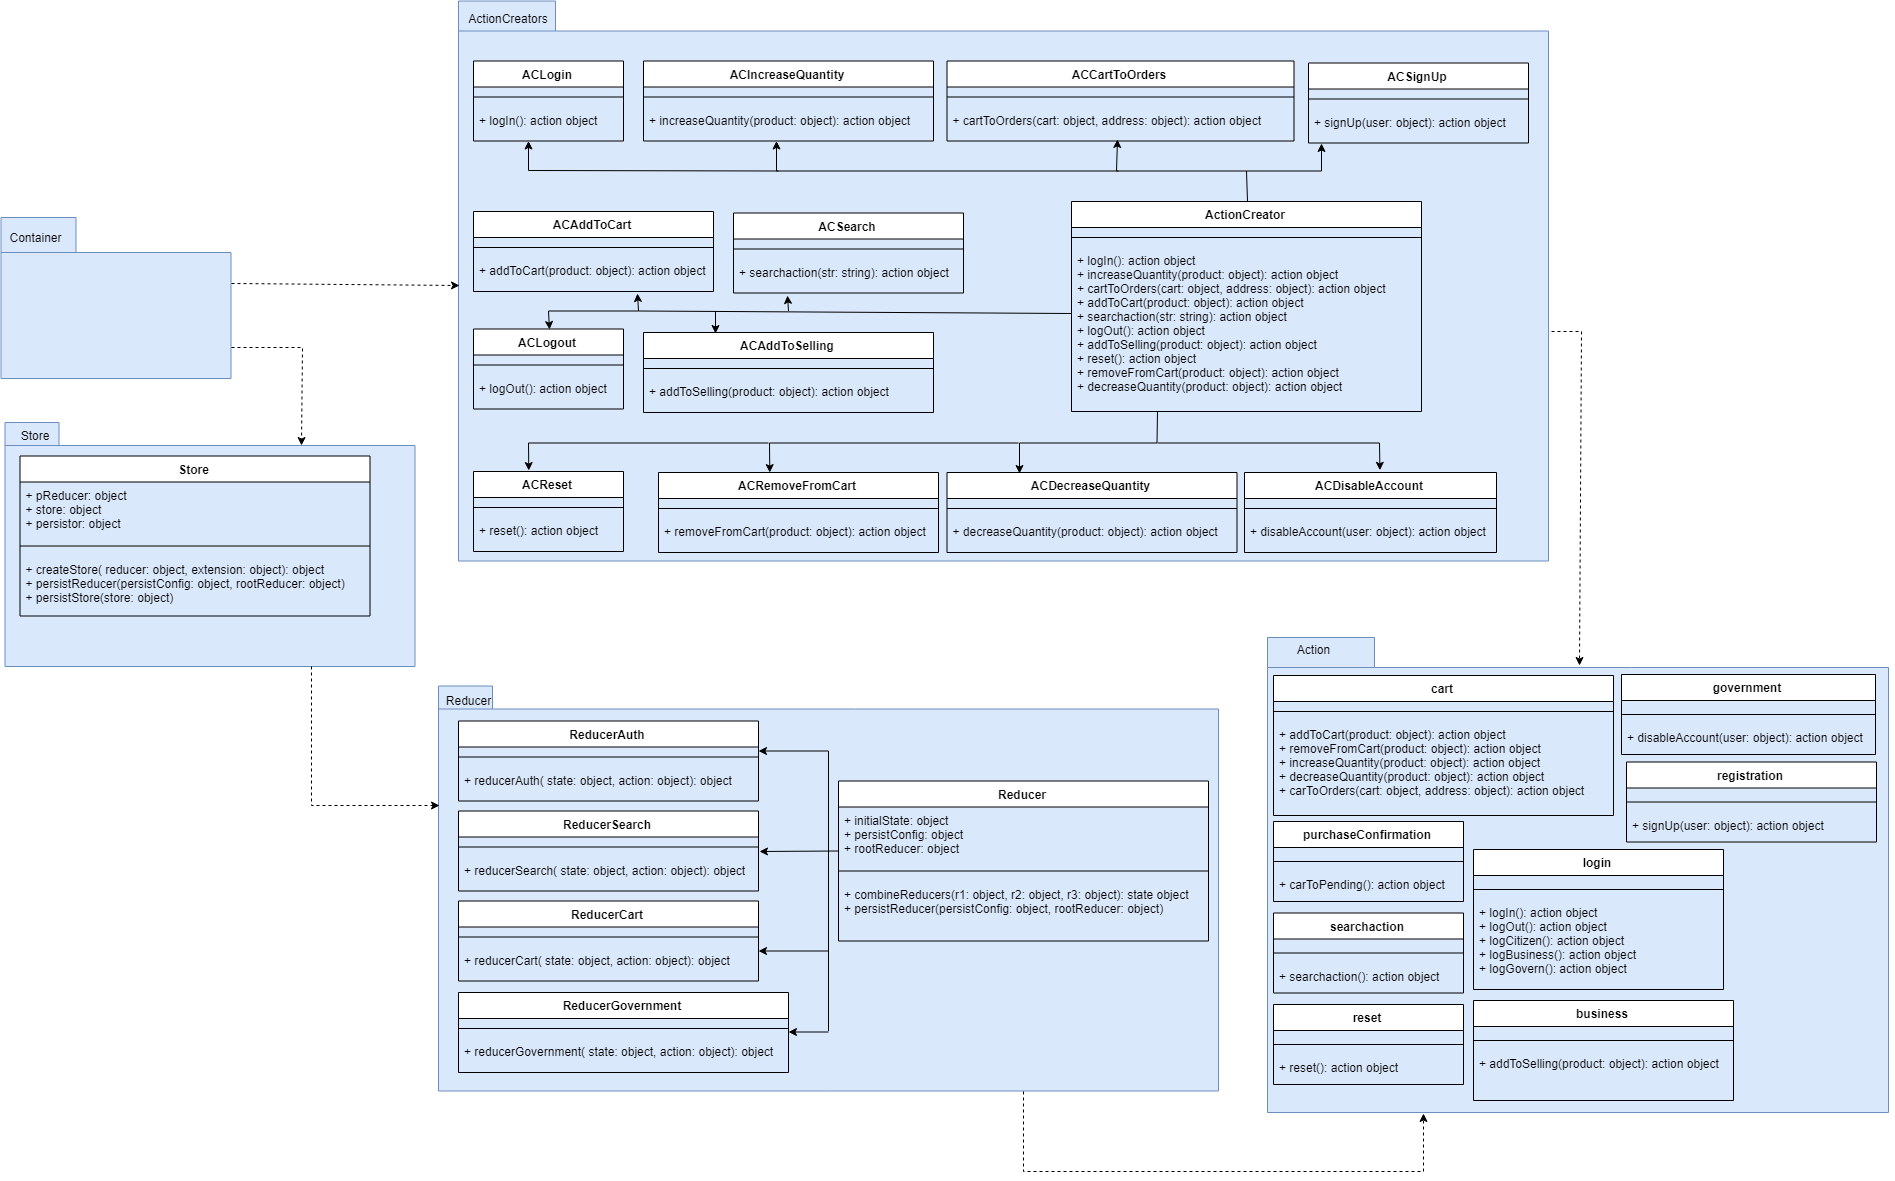
\includegraphics[scale = 0.3]{res/images/ReduxDiagram.png}
		\caption{Redux architecture}
	\end{figure}
\end{landscape}